\chapter{Cognitive walkthough}


\subsection{Creating a cryptographic identity}
A user who is not logged in but who knows the extension is installed, wishes to make use of some of the extensions functionality and his actions result in the creation of a (prerequisite) cryptographic identity.

\begin{desc}

    \item[Action Sequence] \hfill
    
    \begin{enumerate}
        \item Log in to Facebook.
        \item Click on the {\tt [Create Identity]} button.
        \item Enter a password according to the restrictions.
        \item Re-enter password.
    \end{enumerate}
    
    \item[Defense of Credibility] \hfill
        \begin{itemize}
            
            \item The user knows to click the {\tt [Create Identity]} button. We know the user wants to use the extension in some way and is aware that the plugin is installed - it is reasonable to assume that he will look at the toolbar. All other buttons are greyed out, and the process of creating some form of identity/account/profile before using a service is familiar to anyone who has used Facebook, or any other site which requires membership.
            
            \item If the user isn't logged in to Facebook, he knows he must first do so since he will be informed of this on clicking {\tt [Create Identity]}. User will know how to log in to Facebook.
            
            \item User will know how to cancel process as it is clearly marked.
            
            \item Quiting/crashing the browser or canceling will result in a return to the initial state.
            
            \item User will either enter a valid password or be prompted by the restrictions on entering an invalid one, in which case he will then know how to enter a valid password and do so.
            
            \item User will know if he incorrectly re-enters password via an alert.
            
            \item User knows things are OK because an alert informs him the process was successful.
            
        \end{itemize}
\end{desc}

\subsection{Logging in to a cryptographic identity}
A user who is not logged in but has created an identity, wishes to make use of some of the extensions functionality and logs in.

\begin{desc}

    \item[Action Sequence] \hfill
    
    \begin{enumerate}
        \item Log in to Facebook.
        \item Click on the {\tt [Start Encrypted Facebook]} button.
        \item Enter user password.
    \end{enumerate}
    
    \item[Defense of Credibility] \hfill
        \begin{itemize}
            
            \item User knows to click {\tt [Start Encrypted Facebook]} . We know the user wants to use the extension in some way and is aware that the plugin is installed - it is reasonable to assume that he will look at the toolbar. All other buttons are greyed out apart from {\tt [Create Identity]} which he has used before. If he does mistakenly click {\tt [Create Identity]} he will be informed that he already has an identity and that attempting to overwrite it will result in irrevocable data loss. See figure \ref{scn:create}.
            
            \item If the user isn't logged in to Facebook he knows he must first do so since he will be informed of this on clicking {\tt [Start Encrypted Facebook]}. User will know how to log in to Facebook.
            
            \item User will know his password and be able to enter it. In the case that the user doesn't know his password he will know he must create a new one and do so as described in section XXX.
            
        \end{itemize}
\end{desc}

    \begin{figure}[tbph]
        \begin{center}
        
                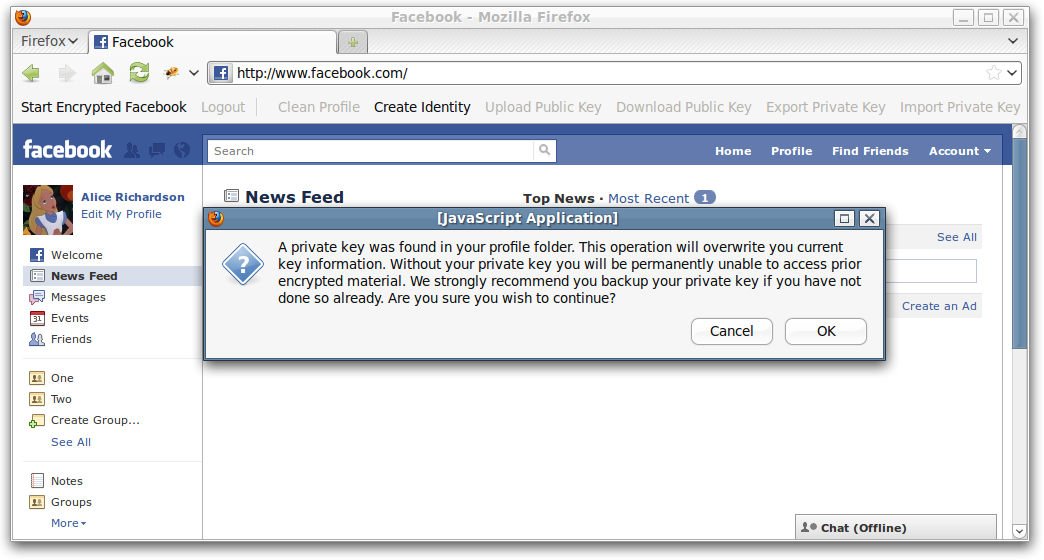
\includegraphics[width=12cm]{screens/create-warning.png}

            \caption{Warning displayed if {\tt [Create Identity]} is mistakely clicked.}
            \label{scn:create}
        \end{center}
    \end{figure}

\subsection{Adding public keys}
A user with no public keys wishes to submit encrypted content. His actions lead to him obtaining one of his intended recipient's public key.

\begin{desc}

    \item[Action Sequence] \hfill
    \begin{enumerate}
        \item Navigate to a friends profile.
        \item Click the {\tt [Add Public Key]} button.
    \end{enumerate}
    
    \item[Defense of Credibility] \hfill
    \begin{itemize}
        \item Assume that a user wishing to perform some encrypted operation knows what process to follow, as demonstrated in sections XXX and XXX. Attempting this process with no public keys will result in a prompt informing the user that they must navigate to a friends profile and click the {\tt [Add Public Key]} button in order to use them as a recipient.
    
        \item Facebook user will be familiar with the process of finding a friends profile and clicking on a button therein.
        
        \item User will know where the {\tt [Add Public Key]} button is since it is clearly labelled and positioned at the top of the page next to several normal Facebook buttons.
        
    \end{itemize}
    
\end{desc}

\subsection{Using the recipient selector control}
A user presented with the recipient selector control wishes to use it to select a large subset of his friends for broadcast encryption, and does so. The user has 406 friends available to select and wants to choose 405 of them.

\begin{desc}

    \item[Action Sequence] \hfill
    \begin{enumerate}
        \item Click the {\tt [Select all]} check button
        \item Deselect the friend who is to be excluded.
        \item Click the {\tt [Submit]} button in the popup window.
    \end{enumerate}
    
    \item[Defense of Credibility] \hfill
        \begin{itemize}
            
            \item User knows that the friend selector is used to select recipients as this is stated clearly abover the control.
            
            \item Users know generally how to select recipients by clicking on them one-by-one and also that they can deselect by clicking an already selected item, since this process of selecting recipients is familiar to them from general Facebook use and the UI control itself is based on Facebook's own. 
            
            \item User knows to click {\tt [Select all]}. The button is visible and clearly labelled; common sense would dictate that selecting all then deselecting one item would be quicker than selecting all 405 items individually.
            
            \item User knows things are OK. After clicking {\tt [Select all]} all items will switch to looking selected in a manner consistent with other controls used by Facebook.
            
            \item User knows how to deselect a friend. Again based on the familiarity with the control from Facebook we assume they are capable of scrolling through the alphabetical list to find their the friend in question.
            
            \item User knows to click {\tt [Submit]}. No button other than cancel is visible on the control, the button is clearly labelled and its appearance and position is based on Facebook's own controls.
            
            \item User knows things are OK as the popup responds to their click by disappearing, identical to the behaviour of a Facebook control.
        
        \end{itemize}
    
\end{desc}